\documentclass[twoside]{book}

% Packages required by doxygen
\usepackage{calc}
\usepackage{doxygen}
\usepackage{graphicx}
\usepackage[utf8]{inputenc}
\usepackage{makeidx}
\usepackage{multicol}
\usepackage{multirow}
\usepackage{textcomp}
\usepackage[table]{xcolor}

% Font selection
\usepackage[T1]{fontenc}
\usepackage{mathptmx}
\usepackage[scaled=.90]{helvet}
\usepackage{courier}
\usepackage{amssymb}
\usepackage{sectsty}
\renewcommand{\familydefault}{\sfdefault}
\allsectionsfont{%
  \fontseries{bc}\selectfont%
  \color{darkgray}%
}
\renewcommand{\DoxyLabelFont}{%
  \fontseries{bc}\selectfont%
  \color{darkgray}%
}

% Page & text layout
\usepackage{geometry}
\geometry{%
  a4paper,%
  top=2.5cm,%
  bottom=2.5cm,%
  left=2.5cm,%
  right=2.5cm%
}
\tolerance=750
\hfuzz=15pt
\hbadness=750
\setlength{\emergencystretch}{15pt}
\setlength{\parindent}{0cm}
\setlength{\parskip}{0.2cm}
\makeatletter
\renewcommand{\paragraph}{%
  \@startsection{paragraph}{4}{0ex}{-1.0ex}{1.0ex}{%
    \normalfont\normalsize\bfseries\SS@parafont%
  }%
}
\renewcommand{\subparagraph}{%
  \@startsection{subparagraph}{5}{0ex}{-1.0ex}{1.0ex}{%
    \normalfont\normalsize\bfseries\SS@subparafont%
  }%
}
\makeatother

% Headers & footers
\usepackage{fancyhdr}
\pagestyle{fancyplain}
\fancyhead[LE]{\fancyplain{}{\bfseries\thepage}}
\fancyhead[CE]{\fancyplain{}{}}
\fancyhead[RE]{\fancyplain{}{\bfseries\leftmark}}
\fancyhead[LO]{\fancyplain{}{\bfseries\rightmark}}
\fancyhead[CO]{\fancyplain{}{}}
\fancyhead[RO]{\fancyplain{}{\bfseries\thepage}}
\fancyfoot[LE]{\fancyplain{}{}}
\fancyfoot[CE]{\fancyplain{}{}}
\fancyfoot[RE]{\fancyplain{}{\bfseries\scriptsize Generated on Mon Jan 6 2014 21\-:10\-:46 for My Project by Doxygen }}
\fancyfoot[LO]{\fancyplain{}{\bfseries\scriptsize Generated on Mon Jan 6 2014 21\-:10\-:46 for My Project by Doxygen }}
\fancyfoot[CO]{\fancyplain{}{}}
\fancyfoot[RO]{\fancyplain{}{}}
\renewcommand{\footrulewidth}{0.4pt}
\renewcommand{\chaptermark}[1]{%
  \markboth{#1}{}%
}
\renewcommand{\sectionmark}[1]{%
  \markright{\thesection\ #1}%
}

% Indices & bibliography
\usepackage{natbib}
\usepackage[titles]{tocloft}
\setcounter{tocdepth}{3}
\setcounter{secnumdepth}{5}
\makeindex

% Hyperlinks (required, but should be loaded last)
\usepackage{ifpdf}
\ifpdf
  \usepackage[pdftex,pagebackref=true]{hyperref}
\else
  \usepackage[ps2pdf,pagebackref=true]{hyperref}
\fi
\hypersetup{%
  colorlinks=true,%
  linkcolor=blue,%
  citecolor=blue,%
  unicode%
}

% Custom commands
\newcommand{\clearemptydoublepage}{%
  \newpage{\pagestyle{empty}\cleardoublepage}%
}


%===== C O N T E N T S =====

\begin{document}

% Titlepage & ToC
\hypersetup{pageanchor=false}
\pagenumbering{roman}
\begin{titlepage}
\vspace*{7cm}
\begin{center}%
{\Large My Project }\\
\vspace*{1cm}
{\large Generated by Doxygen 1.8.6}\\
\vspace*{0.5cm}
{\small Mon Jan 6 2014 21:10:46}\\
\end{center}
\end{titlepage}
\clearemptydoublepage
\tableofcontents
\clearemptydoublepage
\pagenumbering{arabic}
\hypersetup{pageanchor=true}

%--- Begin generated contents ---
\chapter{Hierarchical Index}
\section{Class Hierarchy}
This inheritance list is sorted roughly, but not completely, alphabetically\-:\begin{DoxyCompactList}
\item \contentsline{section}{A\-I}{\pageref{class_a_i}}{}
\begin{DoxyCompactList}
\item \contentsline{section}{test\-K\-I}{\pageref{classtest_k_i}}{}
\end{DoxyCompactList}
\item \contentsline{section}{Board}{\pageref{class_board}}{}
\item \contentsline{section}{Connection}{\pageref{class_connection}}{}
\item \contentsline{section}{Counter}{\pageref{class_counter}}{}
\item \contentsline{section}{Game}{\pageref{class_game}}{}
\item \contentsline{section}{Game\-Logger}{\pageref{class_game_logger}}{}
\item \contentsline{section}{Playing\-Order\-:\-:iterator}{\pageref{class_playing_order_1_1iterator}}{}
\item \contentsline{section}{Move}{\pageref{class_move}}{}
\item \contentsline{section}{Playing\-Order}{\pageref{class_playing_order}}{}
\item Q\-Dialog\begin{DoxyCompactList}
\item \contentsline{section}{Initialize}{\pageref{class_initialize}}{}
\end{DoxyCompactList}
\item Q\-Main\-Window\begin{DoxyCompactList}
\item \contentsline{section}{Main\-Window}{\pageref{class_main_window}}{}
\end{DoxyCompactList}
\item Q\-Widget\begin{DoxyCompactList}
\item \contentsline{section}{Spielbrett}{\pageref{class_spielbrett}}{}
\item \contentsline{section}{Window}{\pageref{class_window}}{}
\end{DoxyCompactList}
\item \contentsline{section}{Round}{\pageref{class_round}}{}
\item \contentsline{section}{Round\-Logger}{\pageref{class_round_logger}}{}
\item \contentsline{section}{Simulation}{\pageref{class_simulation}}{}
\item \contentsline{section}{Simulation\-Logger}{\pageref{class_simulation_logger}}{}
\item \contentsline{section}{State}{\pageref{class_state}}{}
\item \contentsline{section}{U\-I\-E\-X\-E\-C}{\pageref{class_u_i_e_x_e_c}}{}
\item \contentsline{section}{Vector}{\pageref{class_vector}}{}
\begin{DoxyCompactList}
\item \contentsline{section}{City}{\pageref{class_city}}{}
\item \contentsline{section}{Coordinate}{\pageref{class_coordinate}}{}
\item \contentsline{section}{Pawn}{\pageref{class_pawn}}{}
\end{DoxyCompactList}
\end{DoxyCompactList}

\chapter{Class Index}
\section{Class List}
Here are the classes, structs, unions and interfaces with brief descriptions\-:\begin{DoxyCompactList}
\item\contentsline{section}{{\bf A\-I} }{\pageref{class_a_i}}{}
\item\contentsline{section}{{\bf Board} }{\pageref{class_board}}{}
\item\contentsline{section}{{\bf City} }{\pageref{class_city}}{}
\item\contentsline{section}{{\bf Connection} }{\pageref{class_connection}}{}
\item\contentsline{section}{{\bf Coordinate} }{\pageref{class_coordinate}}{}
\item\contentsline{section}{{\bf Counter} }{\pageref{class_counter}}{}
\item\contentsline{section}{{\bf Dynamic\-State} }{\pageref{class_dynamic_state}}{}
\item\contentsline{section}{{\bf Game} }{\pageref{class_game}}{}
\item\contentsline{section}{{\bf Game\-Logger} }{\pageref{class_game_logger}}{}
\item\contentsline{section}{{\bf Initialize} }{\pageref{class_initialize}}{}
\item\contentsline{section}{{\bf Playing\-Order\-::iterator} }{\pageref{class_playing_order_1_1iterator}}{}
\item\contentsline{section}{{\bf Main\-Window} }{\pageref{class_main_window}}{}
\item\contentsline{section}{{\bf Move} }{\pageref{class_move}}{}
\item\contentsline{section}{{\bf Pawn} }{\pageref{class_pawn}}{}
\item\contentsline{section}{{\bf Playing\-Order} }{\pageref{class_playing_order}}{}
\item\contentsline{section}{{\bf Round} }{\pageref{class_round}}{}
\item\contentsline{section}{{\bf Round\-Logger} }{\pageref{class_round_logger}}{}
\item\contentsline{section}{{\bf Simulation} }{\pageref{class_simulation}}{}
\item\contentsline{section}{{\bf Simulation\-Logger} }{\pageref{class_simulation_logger}}{}
\item\contentsline{section}{{\bf Spielbrett} }{\pageref{class_spielbrett}}{}
\item\contentsline{section}{{\bf State} }{\pageref{class_state}}{}
\item\contentsline{section}{{\bf test\-K\-I} }{\pageref{classtest_k_i}}{}
\item\contentsline{section}{{\bf U\-I\-E\-X\-E\-C} }{\pageref{class_u_i_e_x_e_c}}{}
\item\contentsline{section}{{\bf Vector} }{\pageref{class_vector}}{}
\item\contentsline{section}{{\bf Window} }{\pageref{class_window}}{}
\end{DoxyCompactList}

\chapter{Class Documentation}
\hypertarget{class_brett}{\section{Brett Class Reference}
\label{class_brett}\index{Brett@{Brett}}
}
\subsection*{Public Member Functions}
\begin{DoxyCompactItemize}
\item 
\hypertarget{class_brett_a72bbf86800d1f477b9e4625d325e465a}{\hyperlink{class_coordinate}{Coordinate} $\ast$$\ast$$\ast$ {\bfseries gitter\-Anlegen} () const }\label{class_brett_a72bbf86800d1f477b9e4625d325e465a}

\item 
\hypertarget{class_brett_ab326ab4994f8227a6d28a8de09a4d4e5}{const \hyperlink{class_city}{City} $\ast$$\ast$ {\bfseries stadtliste\-Anlegen} () const }\label{class_brett_ab326ab4994f8227a6d28a8de09a4d4e5}

\item 
\hypertarget{class_brett_ae6144255642555208de19a5c967ab145}{\hyperlink{class_verbindung}{Verbindung} $\ast$$\ast$$\ast$$\ast$ {\bfseries kanten\-Anlegen} () const }\label{class_brett_ae6144255642555208de19a5c967ab145}

\item 
\hypertarget{class_brett_af4526c6857f25f88a38e58f025d4baa1}{void {\bfseries Ausgabe} () const }\label{class_brett_af4526c6857f25f88a38e58f025d4baa1}

\item 
\hypertarget{class_brett_ac3511a492cf4f2fab2318fb0e05bd886}{void {\bfseries akt\-Ausgabe} (bool gelegte\-Schienen\mbox{[}M\-A\-X\-\_\-\-X\mbox{]}\mbox{[}M\-A\-X\-\_\-\-Y\mbox{]}\mbox{[}3\mbox{]}) const }\label{class_brett_ac3511a492cf4f2fab2318fb0e05bd886}

\item 
\hypertarget{class_brett_a3d69a2d912d12dd9929a6decffce4c98}{const \hyperlink{class_city}{City} $\ast$const {\bfseries durchsuche\-Liste} (short xkoo, short ykoo) const }\label{class_brett_a3d69a2d912d12dd9929a6decffce4c98}

\item 
\hypertarget{class_brett_a8853bb48bdea6ff1807f32a899a98a65}{const \hyperlink{class_city}{City} $\ast$ {\bfseries get\-Stadt} (short farbe, short nr) const }\label{class_brett_a8853bb48bdea6ff1807f32a899a98a65}

\end{DoxyCompactItemize}
\subsection*{Public Attributes}
\begin{DoxyCompactItemize}
\item 
\hypertarget{class_brett_a1b42422ecdc5c52503fbb247f1d6f838}{const short {\bfseries anzahl\-Staedte}}\label{class_brett_a1b42422ecdc5c52503fbb247f1d6f838}

\item 
\hypertarget{class_brett_a754988bdc50cc03bdf136e3905df252f}{const \hyperlink{class_city}{City} $\ast$const $\ast$const {\bfseries Stadtliste}}\label{class_brett_a754988bdc50cc03bdf136e3905df252f}

\item 
\hypertarget{class_brett_aed2d07eea45ab2dfc98dfad234c50f43}{const \hyperlink{class_coordinate}{Coordinate} $\ast$const $\ast$const \\*
$\ast$const {\bfseries Gitter}}\label{class_brett_aed2d07eea45ab2dfc98dfad234c50f43}

\item 
\hypertarget{class_brett_a9685bc6076da6752c6c619e3798d04c3}{const \hyperlink{class_verbindung}{Verbindung} $\ast$const $\ast$const \\*
$\ast$const $\ast$const {\bfseries Kanten}}\label{class_brett_a9685bc6076da6752c6c619e3798d04c3}

\end{DoxyCompactItemize}


The documentation for this class was generated from the following files\-:\begin{DoxyCompactItemize}
\item 
Brett.\-h\item 
Brett.\-cpp\end{DoxyCompactItemize}

\section{City Class Reference}
\label{class_city}\index{City@{City}}
Inheritance diagram for City\-:\begin{figure}[H]
\begin{center}
\leavevmode
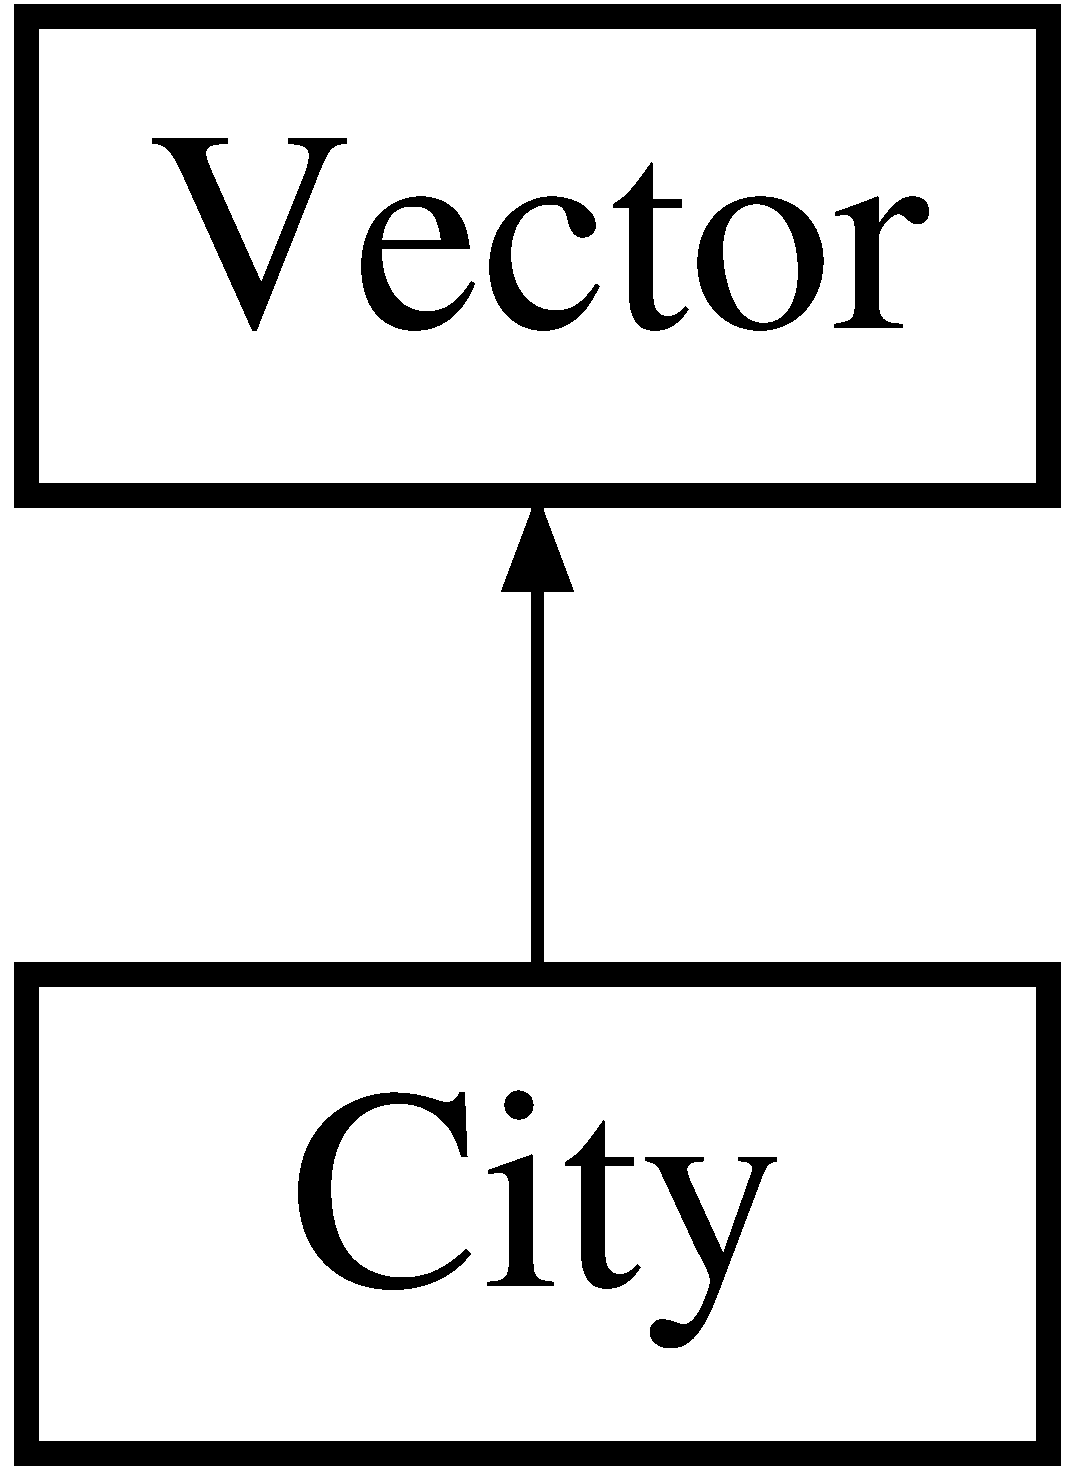
\includegraphics[height=2.000000cm]{class_city}
\end{center}
\end{figure}
\subsection*{Public Member Functions}
\begin{DoxyCompactItemize}
\item 
{\bfseries City} (string name, C\-I\-T\-Y\-C\-O\-L\-O\-U\-R city\-Colour, short number, {\bf Vector} place)\label{class_city_a086f1d9fd30ad0bcedcf72d526cbf365}

\end{DoxyCompactItemize}
\subsection*{Public Attributes}
\begin{DoxyCompactItemize}
\item 
string {\bfseries name}\label{class_city_a38b5e8b9bd4e263434eae0344913d341}

\item 
C\-I\-T\-Y\-C\-O\-L\-O\-U\-R {\bfseries city\-Colour}\label{class_city_a49ce7573be0c500755ffc346399a7ae3}

\item 
short {\bfseries number}\label{class_city_a0fecf97dc1cbd61bb1bd27325decad52}

\end{DoxyCompactItemize}


The documentation for this class was generated from the following files\-:\begin{DoxyCompactItemize}
\item 
hdr/game/City.\-h\item 
src/game/City.\-cpp\end{DoxyCompactItemize}

\hypertarget{class_coordinate}{\section{Coordinate Class Reference}
\label{class_coordinate}\index{Coordinate@{Coordinate}}
}


{\ttfamily \#include $<$Koordinate.\-h$>$}

Inheritance diagram for Coordinate\-:\begin{figure}[H]
\begin{center}
\leavevmode
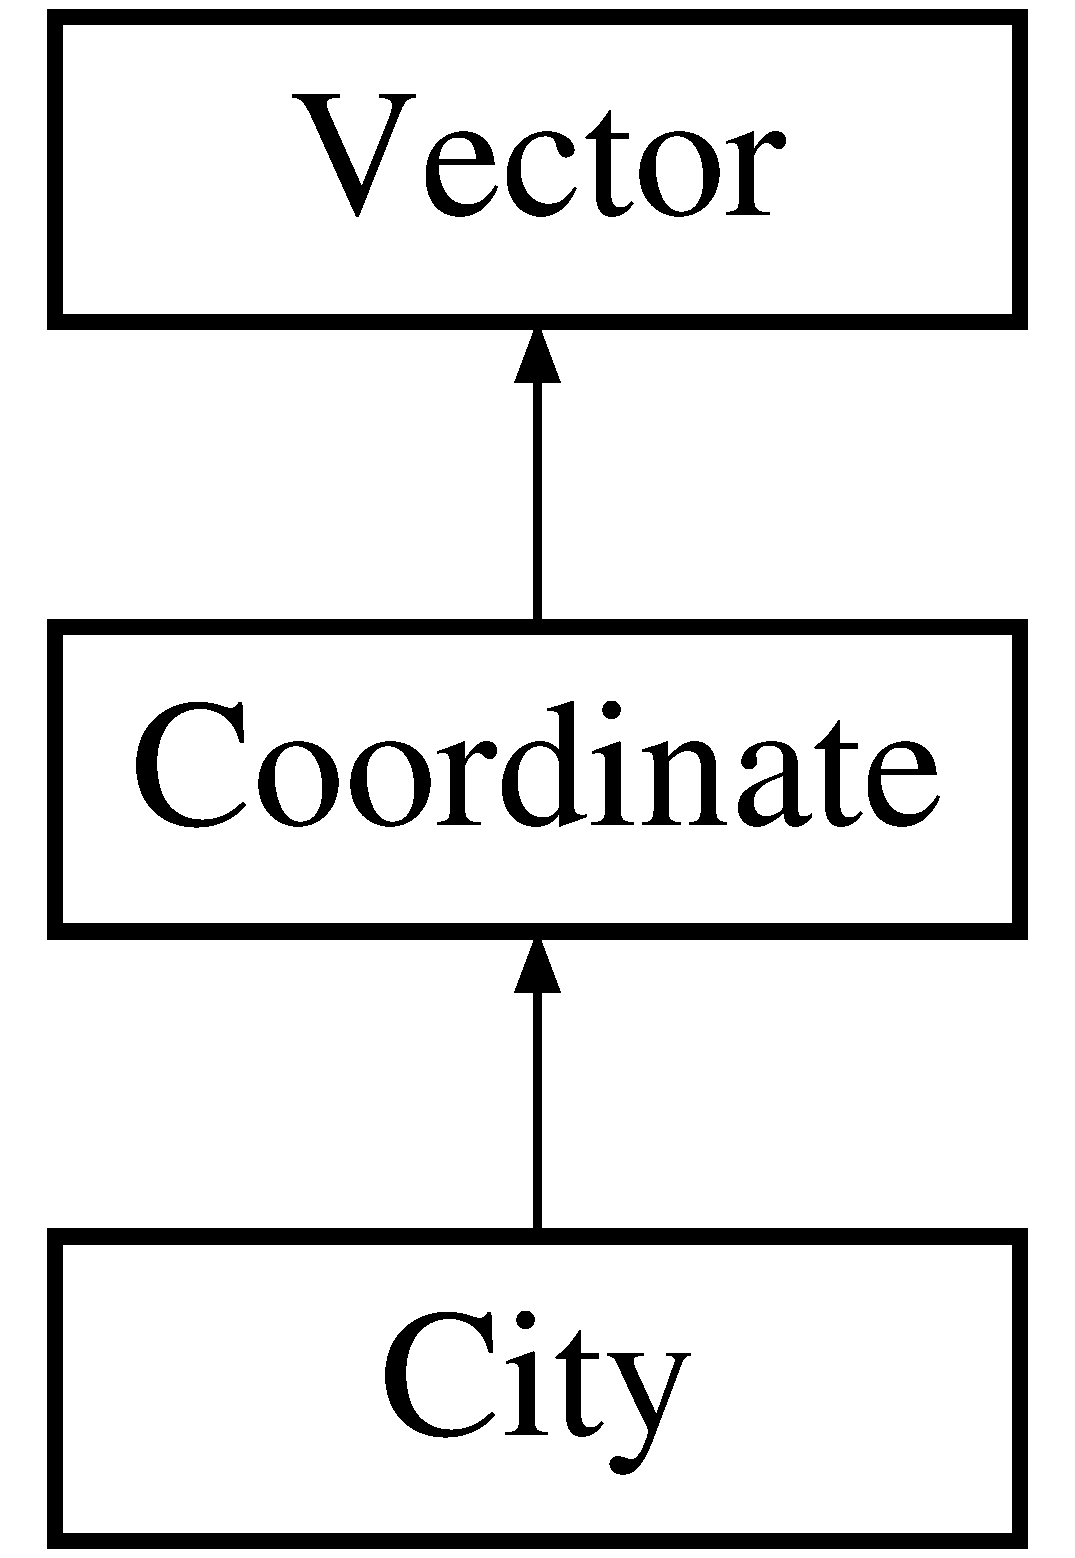
\includegraphics[height=2.000000cm]{class_coordinate}
\end{center}
\end{figure}
\subsection*{Public Member Functions}
\begin{DoxyCompactItemize}
\item 
\hypertarget{class_coordinate_afa539ca7218f25717e25482babf0bfc9}{{\bfseries Coordinate} (short x, short y)}\label{class_coordinate_afa539ca7218f25717e25482babf0bfc9}

\item 
\hypertarget{class_coordinate_a6f212c6c04f0f87e09157cff2092c111}{{\bfseries Coordinate} (short x, short y, const \hyperlink{class_city}{City} \&City\-On\-Coordinate)}\label{class_coordinate_a6f212c6c04f0f87e09157cff2092c111}

\end{DoxyCompactItemize}
\subsection*{Public Attributes}
\begin{DoxyCompactItemize}
\item 
\hypertarget{class_coordinate_a68372ad69c745041d63625c2a9ed4577}{const \hyperlink{class_city}{City} \& {\bfseries vor\-Ort}}\label{class_coordinate_a68372ad69c745041d63625c2a9ed4577}

\item 
\hypertarget{class_coordinate_ac7c3032bcd943e1e0d3576d6ec39745a}{bool {\bfseries Null}}\label{class_coordinate_ac7c3032bcd943e1e0d3576d6ec39745a}

\end{DoxyCompactItemize}


\subsection{Detailed Description}
Objects of this class are coordiantes on the board, where the x-\/axis is parallel to the west-\/east direction and the y-\/axis parallel to the north-\/(south-\/west) direction. The (0,0) coordinate is the most upper left corner of the board. The range of the x-\/values is from 0 to M\-A\-X\-\_\-\-X and the y-\/values from 0 to M\-A\-X\-\_\-\-Y. 

The documentation for this class was generated from the following files\-:\begin{DoxyCompactItemize}
\item 
Koordinate.\-h\item 
Koordinate.\-cpp\end{DoxyCompactItemize}

\section{Game Class Reference}
\label{class_game}\index{Game@{Game}}
\subsection*{Public Member Functions}
\begin{DoxyCompactItemize}
\item 
{\bfseries Game} ({\bf Game\-Logger} $\ast$game\-Logger)\label{class_game_a9f03a276b1af77e70e794ac22ded922e}

\item 
void {\bfseries play} ()\label{class_game_aa333825d0bca80e91e53c7e23f053405}

\end{DoxyCompactItemize}


The documentation for this class was generated from the following files\-:\begin{DoxyCompactItemize}
\item 
hdr/game/Game.\-h\item 
src/game/Game.\-cpp\end{DoxyCompactItemize}

\hypertarget{class_k_ispieler}{\section{K\-Ispieler Class Reference}
\label{class_k_ispieler}\index{K\-Ispieler@{K\-Ispieler}}
}
Inheritance diagram for K\-Ispieler\-:\begin{figure}[H]
\begin{center}
\leavevmode
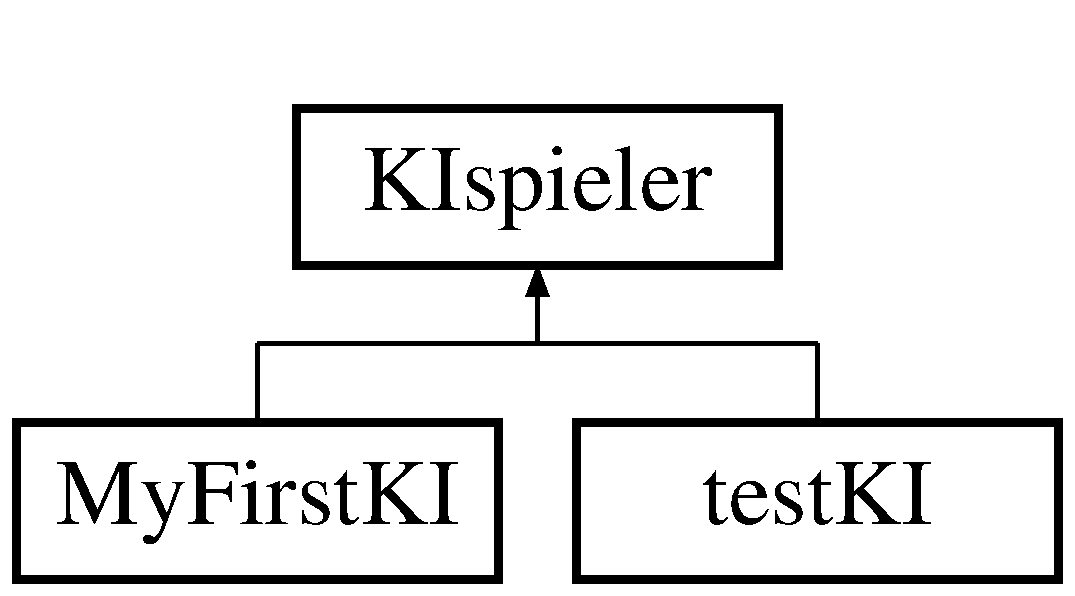
\includegraphics[height=2.000000cm]{class_k_ispieler}
\end{center}
\end{figure}
\subsection*{Public Member Functions}
\begin{DoxyCompactItemize}
\item 
\hypertarget{class_k_ispieler_a236f6bcb632fcf5584f23668843f28c3}{{\bfseries K\-Ispieler} (short spielerfarbe)}\label{class_k_ispieler_a236f6bcb632fcf5584f23668843f28c3}

\end{DoxyCompactItemize}
\subsection*{Public Attributes}
\begin{DoxyCompactItemize}
\item 
\hypertarget{class_k_ispieler_a57f2acc7c2c2f19b5f8db7912e8550a8}{const short {\bfseries spielerfarbe}}\label{class_k_ispieler_a57f2acc7c2c2f19b5f8db7912e8550a8}

\item 
\hypertarget{class_k_ispieler_a9bb08608afb5701e852435879ba60369}{string {\bfseries programmierer}}\label{class_k_ispieler_a9bb08608afb5701e852435879ba60369}

\end{DoxyCompactItemize}
\subsection*{Protected Member Functions}
\begin{DoxyCompactItemize}
\item 
\hypertarget{class_k_ispieler_a6007b5100ed30faaae57c13c71a61e39}{virtual \hyperlink{class_move}{Move} {\bfseries zug} (\hyperlink{class_zustand}{Zustand} \&aktuell) const =0}\label{class_k_ispieler_a6007b5100ed30faaae57c13c71a61e39}

\item 
\hypertarget{class_k_ispieler_ad91a31127d0a9f8a22c157f6d8c9cfcf}{virtual \hyperlink{class_vector}{Vector} {\bfseries poeppel\-Setzen} (\hyperlink{class_zustand}{Zustand} \&aktuell) const =0}\label{class_k_ispieler_ad91a31127d0a9f8a22c157f6d8c9cfcf}

\end{DoxyCompactItemize}
\subsection*{Protected Attributes}
\begin{DoxyCompactItemize}
\item 
\hypertarget{class_k_ispieler_a088a3fc4fcfa576b785a067e87f3a7e7}{const \hyperlink{class_city}{City} $\ast$$\ast$ {\bfseries handkarten}}\label{class_k_ispieler_a088a3fc4fcfa576b785a067e87f3a7e7}

\end{DoxyCompactItemize}
\subsection*{Friends}
\begin{DoxyCompactItemize}
\item 
\hypertarget{class_k_ispieler_aa2fab026580d6f14280c2ffb8063a314}{class {\bfseries Game}}\label{class_k_ispieler_aa2fab026580d6f14280c2ffb8063a314}

\end{DoxyCompactItemize}


The documentation for this class was generated from the following files\-:\begin{DoxyCompactItemize}
\item 
K\-Ispieler.\-h\item 
K\-Ispieler.\-cpp\end{DoxyCompactItemize}

\hypertarget{class_move}{\section{Move Class Reference}
\label{class_move}\index{Move@{Move}}
}
\subsection*{Public Member Functions}
\begin{DoxyCompactItemize}
\item 
\hypertarget{class_move_adad54af2a6af52e8a1b37cc0c28a9c03}{{\bfseries Move} (short spielerfarbe, const \hyperlink{class_verbindung}{Verbindung} $\ast$belegt1, const \hyperlink{class_verbindung}{Verbindung} $\ast$belegt2)}\label{class_move_adad54af2a6af52e8a1b37cc0c28a9c03}

\item 
\hypertarget{class_move_a4a681053577ea9b245e8794c427fe910}{bool {\bfseries gueltig} (\hyperlink{class_zustand}{Zustand}, short)}\label{class_move_a4a681053577ea9b245e8794c427fe910}

\item 
\hypertarget{class_move_a982e038b4f43336bf8396d8e63f9cebb}{void {\bfseries ausfuehren} (\hyperlink{class_zustand}{Zustand} \&) const }\label{class_move_a982e038b4f43336bf8396d8e63f9cebb}

\item 
\hypertarget{class_move_a5fd65957977d9e30fd8898fa4a14ac56}{void {\bfseries dump} () const }\label{class_move_a5fd65957977d9e30fd8898fa4a14ac56}

\item 
\hypertarget{class_move_a2cae41881447ddc9496cff2800ce01e2}{\hyperlink{class_move}{Move} \& {\bfseries operator=} (const \hyperlink{class_move}{Move} \&zuweisung)}\label{class_move_a2cae41881447ddc9496cff2800ce01e2}

\end{DoxyCompactItemize}


The documentation for this class was generated from the following files\-:\begin{DoxyCompactItemize}
\item 
Move.\-h\item 
Move.\-cpp\end{DoxyCompactItemize}

\hypertarget{class_my_first_k_i}{\section{My\-First\-K\-I Class Reference}
\label{class_my_first_k_i}\index{My\-First\-K\-I@{My\-First\-K\-I}}
}
Inheritance diagram for My\-First\-K\-I\-:\begin{figure}[H]
\begin{center}
\leavevmode
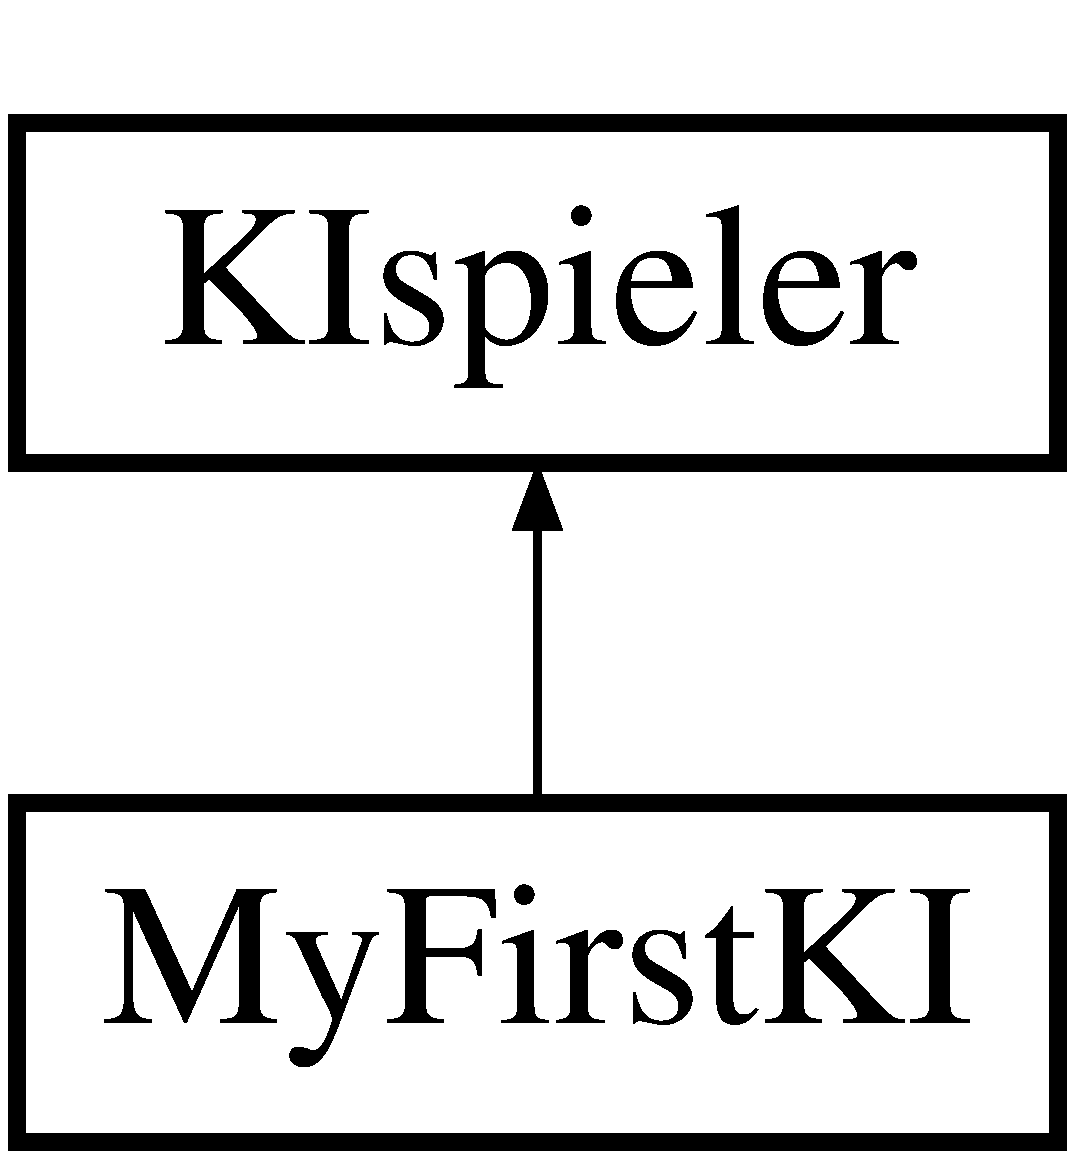
\includegraphics[height=2.000000cm]{class_my_first_k_i}
\end{center}
\end{figure}
\subsection*{Public Member Functions}
\begin{DoxyCompactItemize}
\item 
\hypertarget{class_my_first_k_i_ac75297663481129c68bfd32adcbc3192}{{\bfseries My\-First\-K\-I} (short spielerfarbe)}\label{class_my_first_k_i_ac75297663481129c68bfd32adcbc3192}

\end{DoxyCompactItemize}
\subsection*{Additional Inherited Members}


The documentation for this class was generated from the following files\-:\begin{DoxyCompactItemize}
\item 
My\-First\-K\-I.\-h\item 
My\-First\-K\-I.\-cpp\end{DoxyCompactItemize}

\hypertarget{class_poeppel}{\section{Poeppel Class Reference}
\label{class_poeppel}\index{Poeppel@{Poeppel}}
}
\subsection*{Public Member Functions}
\begin{DoxyCompactItemize}
\item 
\hypertarget{class_poeppel_ae04ebf45f513174d7b45b75eccf025b0}{{\bfseries Poeppel} (short farb, \hyperlink{class_vector}{Vector} pos)}\label{class_poeppel_ae04ebf45f513174d7b45b75eccf025b0}

\item 
\hypertarget{class_poeppel_a253cd856015b757908a07bb88cf72d48}{{\bfseries Poeppel} (const \hyperlink{class_poeppel}{Poeppel} \&copy)}\label{class_poeppel_a253cd856015b757908a07bb88cf72d48}

\end{DoxyCompactItemize}
\subsection*{Public Attributes}
\begin{DoxyCompactItemize}
\item 
\hypertarget{class_poeppel_a3bd9c0c24f0942c45860456d74e1d6c3}{short {\bfseries schienennetznummer}}\label{class_poeppel_a3bd9c0c24f0942c45860456d74e1d6c3}

\item 
\hypertarget{class_poeppel_a6ecf97e3a19a3bf8108a105f0f2603ca}{const short {\bfseries spielerfarbe}}\label{class_poeppel_a6ecf97e3a19a3bf8108a105f0f2603ca}

\item 
\hypertarget{class_poeppel_a45360c7e6518f8ce80ab681f90a58824}{const \hyperlink{class_vector}{Vector} {\bfseries startposition}}\label{class_poeppel_a45360c7e6518f8ce80ab681f90a58824}

\end{DoxyCompactItemize}


The documentation for this class was generated from the following files\-:\begin{DoxyCompactItemize}
\item 
Poeppel.\-h\item 
Poeppel.\-cpp\end{DoxyCompactItemize}

\section{test\-K\-I Class Reference}
\label{classtest_k_i}\index{test\-K\-I@{test\-K\-I}}
Inheritance diagram for test\-K\-I\-:\begin{figure}[H]
\begin{center}
\leavevmode
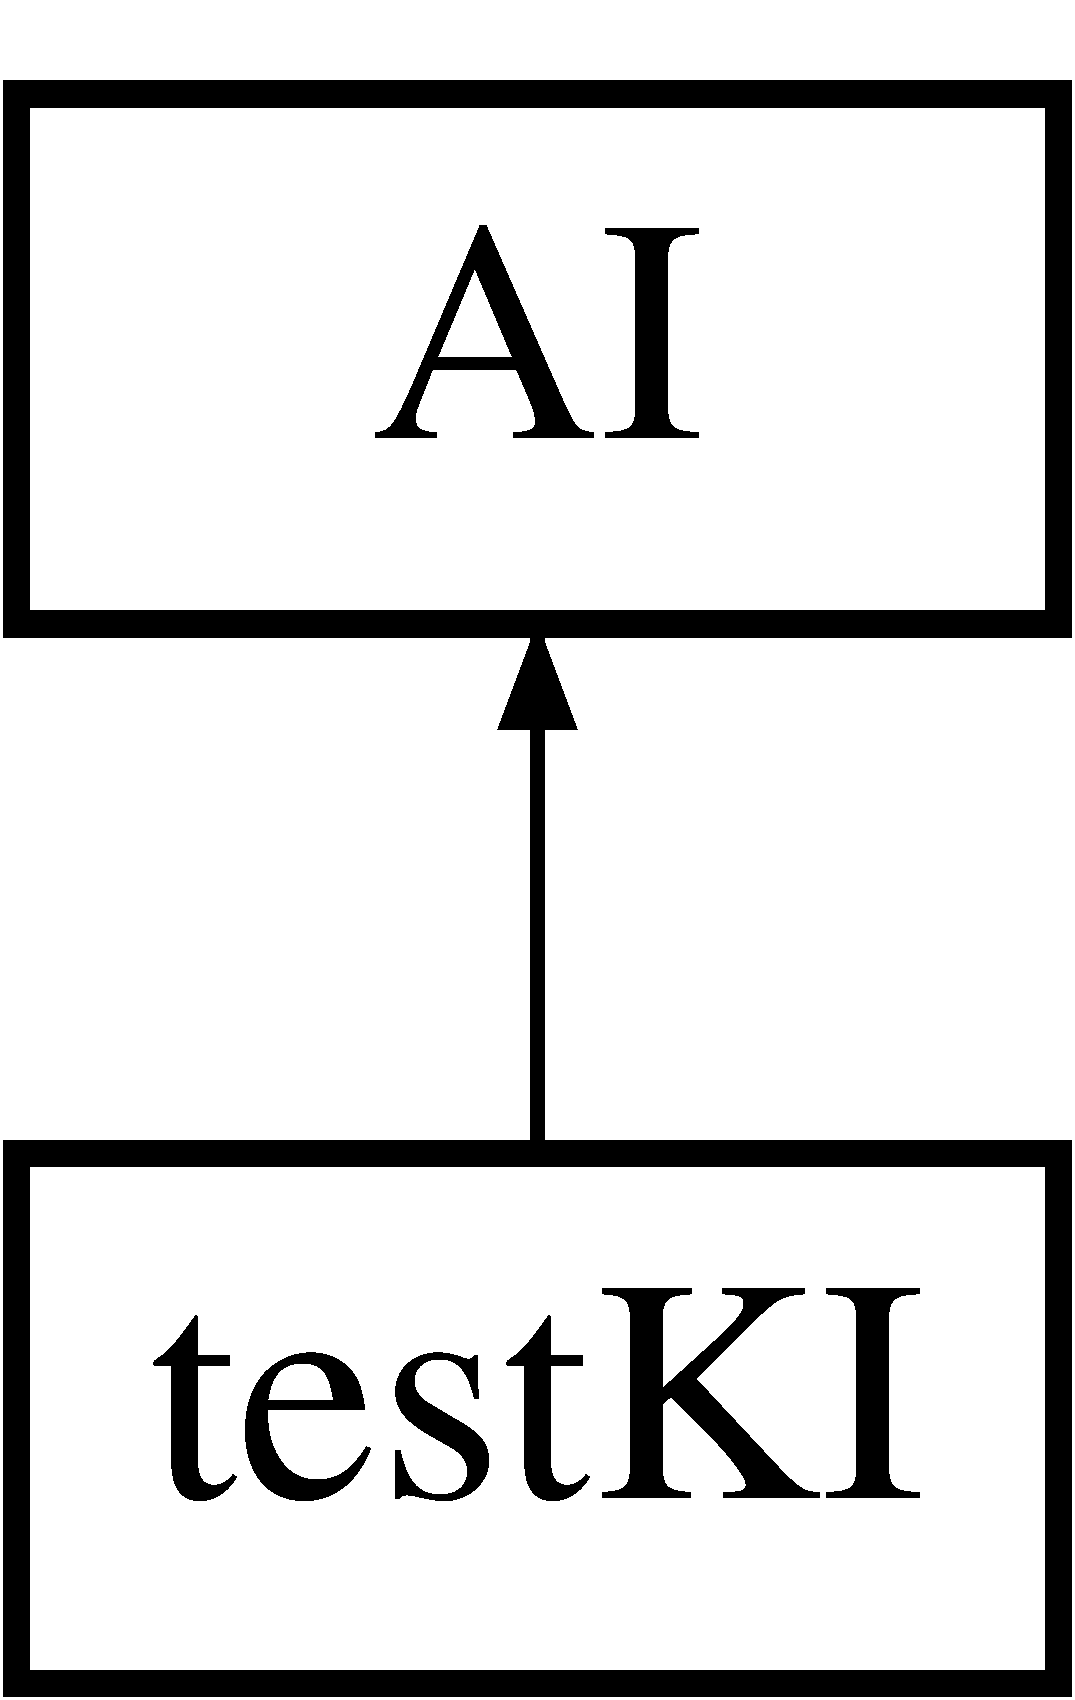
\includegraphics[height=2.000000cm]{classtest_k_i}
\end{center}
\end{figure}
\subsection*{Public Member Functions}
\begin{DoxyCompactItemize}
\item 
{\bfseries test\-K\-I} (P\-L\-A\-Y\-E\-R\-C\-O\-L\-O\-R farbe)\label{classtest_k_i_ac9ced0085410300732bb3103db6934e9}

\item 
{\bf Move} {\bf do\-Move} ({\bf State} \&aktuell)
\item 
{\bf Vector} {\bf set\-Pawn} ({\bf State} \&aktuell)
\item 
bool {\bf count\-Points} ({\bf State} \&, std\-::vector$<$ {\bf Connection} $\ast$ $>$)
\item 
void {\bf gather\-Information\-End\-Of\-Round} (const {\bf Round\-Logger} $\ast$)
\item 
{\bf Vector} {\bfseries get\-Naechster\-Punkt\-Zu} ({\bf Vector}, {\bf State}) const \label{classtest_k_i_ae5c4cfdc479bb706a9adb84d41dff707}

\end{DoxyCompactItemize}
\subsection*{Static Public Member Functions}
\begin{DoxyCompactItemize}
\item 
static short {\bfseries sign} (short)\label{classtest_k_i_a22f65151709965a8d75c82ebc34f3c14}

\end{DoxyCompactItemize}
\subsection*{Additional Inherited Members}


\subsection{Member Function Documentation}
\index{test\-K\-I@{test\-K\-I}!count\-Points@{count\-Points}}
\index{count\-Points@{count\-Points}!testKI@{test\-K\-I}}
\subsubsection[{count\-Points}]{\setlength{\rightskip}{0pt plus 5cm}bool test\-K\-I\-::count\-Points (
\begin{DoxyParamCaption}
\item[{{\bf State} \&}]{current\-State, }
\item[{std\-::vector$<$ {\bf Connection} $\ast$ $>$}]{path}
\end{DoxyParamCaption}
)\hspace{0.3cm}{\ttfamily [inline]}, {\ttfamily [virtual]}}\label{classtest_k_i_aa63e7bbbebbd5a3d01b60ccf7c9bf5f9}
Here you can count your minus points at the end of each round. If you want to do so, you have to return true. For the beginning it is okay, if you just return false. Then the gamemaster will count the minuspoints. He counts in most cases the minimum of minuspoints you get, however in some cases the algorithm doesn't evaluate the best value. 

Implements {\bf A\-I} \doxyref{}{p.}{class_a_i_a17ab5d8748cd5b8afc7e73c42ef12fb3}.

\index{test\-K\-I@{test\-K\-I}!do\-Move@{do\-Move}}
\index{do\-Move@{do\-Move}!testKI@{test\-K\-I}}
\subsubsection[{do\-Move}]{\setlength{\rightskip}{0pt plus 5cm}{\bf Move} test\-K\-I\-::do\-Move (
\begin{DoxyParamCaption}
\item[{{\bf State} \&}]{aktuell}
\end{DoxyParamCaption}
)\hspace{0.3cm}{\ttfamily [virtual]}}\label{classtest_k_i_ad7de22d69a58dca460270955eff84e76}
Inside this methode you calculate your next move in the game. 

Implements {\bf A\-I} \doxyref{}{p.}{class_a_i_a79bb57422a56d4e941c538f2c7491953}.

\index{test\-K\-I@{test\-K\-I}!gather\-Information\-End\-Of\-Round@{gather\-Information\-End\-Of\-Round}}
\index{gather\-Information\-End\-Of\-Round@{gather\-Information\-End\-Of\-Round}!testKI@{test\-K\-I}}
\subsubsection[{gather\-Information\-End\-Of\-Round}]{\setlength{\rightskip}{0pt plus 5cm}void test\-K\-I\-::gather\-Information\-End\-Of\-Round (
\begin{DoxyParamCaption}
\item[{const {\bf Round\-Logger} $\ast$}]{current\-Infos}
\end{DoxyParamCaption}
)\hspace{0.3cm}{\ttfamily [inline]}, {\ttfamily [virtual]}}\label{classtest_k_i_ad08fbc5e5f7a5686e02698b604feabb8}
At the end of each round you can take a look at the whole game and the playing cards of your opponents. This can be usefull, if you want to figure out there strategy and react to that over a simulation period. 

Implements {\bf A\-I} \doxyref{}{p.}{class_a_i_a8565a9ef04ac4f9913913c99f65213b2}.

\index{test\-K\-I@{test\-K\-I}!set\-Pawn@{set\-Pawn}}
\index{set\-Pawn@{set\-Pawn}!testKI@{test\-K\-I}}
\subsubsection[{set\-Pawn}]{\setlength{\rightskip}{0pt plus 5cm}{\bf Vector} test\-K\-I\-::set\-Pawn (
\begin{DoxyParamCaption}
\item[{{\bf State} \&}]{aktuell}
\end{DoxyParamCaption}
)\hspace{0.3cm}{\ttfamily [virtual]}}\label{classtest_k_i_a209548aefee567d45db4bb449321aa55}
At the beginning of each round you have to define your starting position of your pawn. 

Implements {\bf A\-I} \doxyref{}{p.}{class_a_i_a0fbc5b7d4230575baf80217d0c250cc9}.



The documentation for this class was generated from the following files\-:\begin{DoxyCompactItemize}
\item 
hdr/ai/test\-K\-I.\-h\item 
src/ai/test\-K\-I.\-cpp\end{DoxyCompactItemize}

\section{Vector Class Reference}
\label{class_vector}\index{Vector@{Vector}}


{\ttfamily \#include $<$Vector.\-h$>$}

Inheritance diagram for Vector\-:\begin{figure}[H]
\begin{center}
\leavevmode
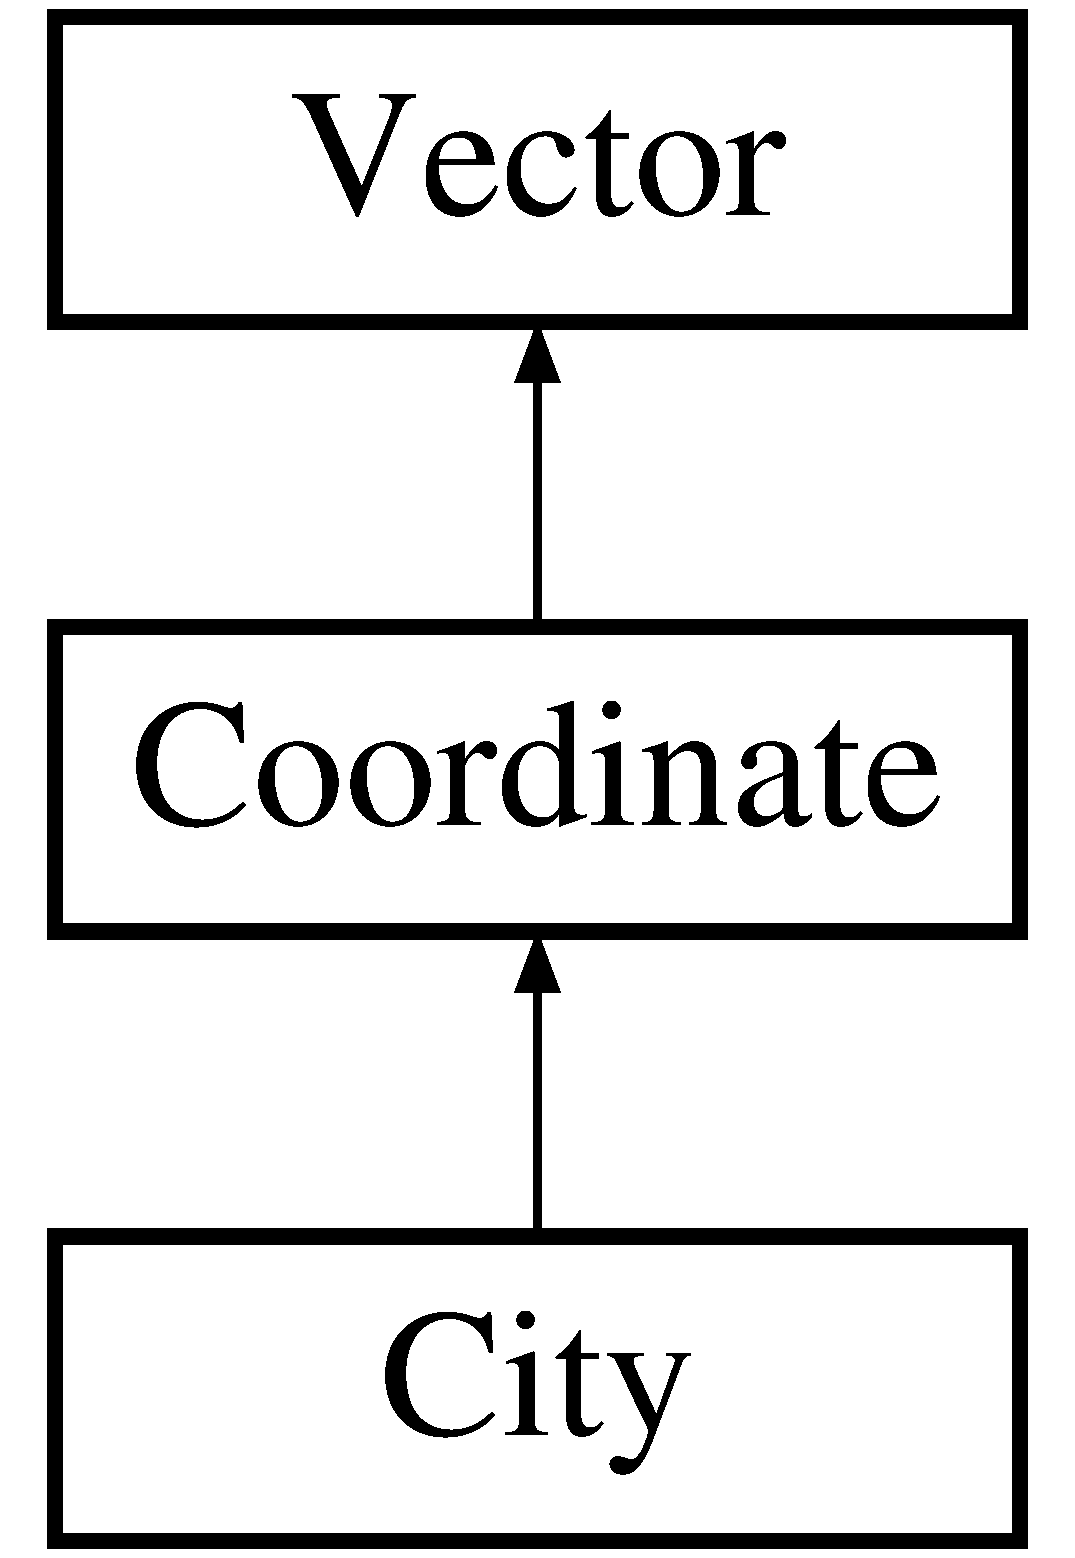
\includegraphics[height=2.000000cm]{class_vector}
\end{center}
\end{figure}
\subsection*{Public Member Functions}
\begin{DoxyCompactItemize}
\item 
{\bfseries Vector} (short x, short y)\label{class_vector_adbd8debb014cdfb97224a1d57b8d44a6}

\item 
{\bf Vector} {\bfseries operator-\/} (const {\bf Vector}) const \label{class_vector_aa283b61aaf9c0895288df72a56ac8899}

\item 
{\bf Vector} {\bfseries operator+} (const {\bf Vector}) const \label{class_vector_aad6d0d53c60571b1bbc52f1ecbc7b0c0}

\item 
short {\bf distance} () const 
\item 
void {\bf dump} () const 
\end{DoxyCompactItemize}
\subsection*{Public Attributes}
\begin{DoxyCompactItemize}
\item 
short {\bfseries x}\label{class_vector_a6784dd08f2e63d06fd376ddaa641f54c}

\item 
short {\bfseries y}\label{class_vector_a17bf7f9707a6ba166c08472377c8c732}

\end{DoxyCompactItemize}


\subsection{Detailed Description}
An object of the class \doxyref{Vector}{p.}{class_vector} represents a 2-\/dimensional vector with two integer values. It is a vector referenced to the board of the game. 

\subsection{Member Function Documentation}
\index{Vector@{Vector}!distance@{distance}}
\index{distance@{distance}!Vector@{Vector}}
\subsubsection[{distance}]{\setlength{\rightskip}{0pt plus 5cm}short Vector\-::distance (
\begin{DoxyParamCaption}
{}
\end{DoxyParamCaption}
) const}\label{class_vector_ac57f428cc1e03ce8cd3c9f6c98a8336f}
Determines a non-\/negative integer, that represents the distance on the board in terms of steps. \-: This distance doesn't represent the number of steps, because it doesn't take care of bridges/tunnels! \index{Vector@{Vector}!dump@{dump}}
\index{dump@{dump}!Vector@{Vector}}
\subsubsection[{dump}]{\setlength{\rightskip}{0pt plus 5cm}void Vector\-::dump (
\begin{DoxyParamCaption}
{}
\end{DoxyParamCaption}
) const\hspace{0.3cm}{\ttfamily [inline]}}\label{class_vector_a50123df9754e508f3d4aa7cb72f38905}
Dumps the values of the vector on the standard stream. 

The documentation for this class was generated from the following files\-:\begin{DoxyCompactItemize}
\item 
game/header/Vector.\-h\item 
game/source/Vector.\-cpp\end{DoxyCompactItemize}

\hypertarget{class_verbindung}{\section{Verbindung Class Reference}
\label{class_verbindung}\index{Verbindung@{Verbindung}}
}
\subsection*{Public Member Functions}
\begin{DoxyCompactItemize}
\item 
\hypertarget{class_verbindung_a1daa504a0c8a9b09667426d2eb79ff1c}{{\bfseries Verbindung} (const \hyperlink{class_coordinate}{Coordinate} \&erste, const \hyperlink{class_coordinate}{Coordinate} \&zweite, bool Hindernis)}\label{class_verbindung_a1daa504a0c8a9b09667426d2eb79ff1c}

\item 
\hypertarget{class_verbindung_a75c826febffaeb8e1a1e4fca6622620f}{const \hyperlink{class_verbindung}{Verbindung} \& {\bfseries operator=} (const \hyperlink{class_verbindung}{Verbindung} \&) const }\label{class_verbindung_a75c826febffaeb8e1a1e4fca6622620f}

\end{DoxyCompactItemize}
\subsection*{Public Attributes}
\begin{DoxyCompactItemize}
\item 
\hypertarget{class_verbindung_a6754cb8101160c165f1910581cf924bc}{const \hyperlink{class_coordinate}{Coordinate} \& {\bfseries first}}\label{class_verbindung_a6754cb8101160c165f1910581cf924bc}

\item 
\hypertarget{class_verbindung_a7fd47daefa46c0329003441cc877eb2d}{const \hyperlink{class_coordinate}{Coordinate} \& {\bfseries second}}\label{class_verbindung_a7fd47daefa46c0329003441cc877eb2d}

\item 
\hypertarget{class_verbindung_a28b2efafed8248ecfc41d5097046784b}{const \hyperlink{class_vector}{Vector} {\bfseries richtung}}\label{class_verbindung_a28b2efafed8248ecfc41d5097046784b}

\item 
\hypertarget{class_verbindung_abcf800621e1099ee1c70aef06f43a663}{bool {\bfseries hindernis}}\label{class_verbindung_abcf800621e1099ee1c70aef06f43a663}

\end{DoxyCompactItemize}


The documentation for this class was generated from the following files\-:\begin{DoxyCompactItemize}
\item 
Verbindung.\-h\item 
Verbindung.\-cpp\end{DoxyCompactItemize}

\hypertarget{class_zustand}{\section{Zustand Class Reference}
\label{class_zustand}\index{Zustand@{Zustand}}
}
\subsection*{Public Member Functions}
\begin{DoxyCompactItemize}
\item 
\hypertarget{class_zustand_a410324ad5c01c1127abecdc679614558}{{\bfseries Zustand} (\hyperlink{class_brett}{Brett} \&Spielbrett)}\label{class_zustand_a410324ad5c01c1127abecdc679614558}

\item 
\hypertarget{class_zustand_aa4ba7f6949af30626a99ce39abed0530}{{\bfseries Zustand} (const \hyperlink{class_zustand}{Zustand} \&)}\label{class_zustand_aa4ba7f6949af30626a99ce39abed0530}

\item 
\hypertarget{class_zustand_a7c423e5ed9d1710d23dc42ae4cea3fdd}{\hyperlink{class_poeppel}{Poeppel} {\bfseries get\-Poeppel} (const short spielerfarbe) const }\label{class_zustand_a7c423e5ed9d1710d23dc42ae4cea3fdd}

\item 
\hypertarget{class_zustand_a6fec4433f91b9fd1abd3ce4d3b2ee562}{bool {\bfseries schienen\-Netz\-Nummer\-Von\-\_\-\-Ist\-\_\-} (const \hyperlink{class_verbindung}{Verbindung} \&, const short schienennr) const }\label{class_zustand_a6fec4433f91b9fd1abd3ce4d3b2ee562}

\item 
\hypertarget{class_zustand_ab88277c8bc572aa6b76f96a05471c6e4}{short {\bfseries get\-Schienen\-Netz\-Nummer} (const \hyperlink{class_vector}{Vector} \&koo) const }\label{class_zustand_ab88277c8bc572aa6b76f96a05471c6e4}

\item 
\hypertarget{class_zustand_af079579ce91bf5cde6b9d1e00d157399}{void {\bfseries set\-Schienen\-Netz\-Nummer} (const \hyperlink{class_coordinate}{Coordinate} \&koo, const short nr)}\label{class_zustand_af079579ce91bf5cde6b9d1e00d157399}

\item 
\hypertarget{class_zustand_a92003ddf9471d768ef544957474ce168}{void {\bfseries set\-Schiene} (const \hyperlink{class_verbindung}{Verbindung} \&)}\label{class_zustand_a92003ddf9471d768ef544957474ce168}

\item 
\hypertarget{class_zustand_adcae9b5b3c032ceefdaac7c49fe6674f}{void {\bfseries reset\-Nr\-\_\-\-Zu\-Nr\-\_\-} (const short, const short)}\label{class_zustand_adcae9b5b3c032ceefdaac7c49fe6674f}

\item 
\hypertarget{class_zustand_a326f241888c2a8897c934d25a8d643b9}{void {\bfseries schiene\-Legen} (const \hyperlink{class_verbindung}{Verbindung} \&)}\label{class_zustand_a326f241888c2a8897c934d25a8d643b9}

\item 
\hypertarget{class_zustand_a1a0b109709853779b7fd4fa720dadbc3}{const \hyperlink{class_verbindung}{Verbindung} \& {\bfseries get\-Verbindung} (\hyperlink{class_vector}{Vector} a, \hyperlink{class_vector}{Vector} b) const }\label{class_zustand_a1a0b109709853779b7fd4fa720dadbc3}

\item 
\hypertarget{class_zustand_aaf796c394dae78069ef3891d75e53e67}{void {\bfseries add\-Poeppel} (\hyperlink{class_poeppel}{Poeppel} insert)}\label{class_zustand_aaf796c394dae78069ef3891d75e53e67}

\item 
\hypertarget{class_zustand_a948904b2d1d4da0868a6a4f063923f3f}{void {\bfseries reset\-All} ()}\label{class_zustand_a948904b2d1d4da0868a6a4f063923f3f}

\end{DoxyCompactItemize}
\subsection*{Static Public Member Functions}
\begin{DoxyCompactItemize}
\item 
\hypertarget{class_zustand_a5962a9e80efba68d605dda8a20431200}{static short {\bfseries Richtungs\-Wert} (const \hyperlink{class_vector}{Vector} \&)}\label{class_zustand_a5962a9e80efba68d605dda8a20431200}

\end{DoxyCompactItemize}
\subsection*{Public Attributes}
\begin{DoxyCompactItemize}
\item 
\hypertarget{class_zustand_ab3a05b260a1c02bad4d110d6026f2800}{short {\bfseries schienen\-Netz\-Nummer} \mbox{[}M\-A\-X\-\_\-\-X\mbox{]}\mbox{[}M\-A\-X\-\_\-\-Y\mbox{]}}\label{class_zustand_ab3a05b260a1c02bad4d110d6026f2800}

\item 
\hypertarget{class_zustand_a425b7daee28c7df0c7a8a778226ee5a7}{bool {\bfseries schiene\-Gelegt} \mbox{[}M\-A\-X\-\_\-\-X\mbox{]}\mbox{[}M\-A\-X\-\_\-\-Y\mbox{]}\mbox{[}3\mbox{]}}\label{class_zustand_a425b7daee28c7df0c7a8a778226ee5a7}

\item 
\hypertarget{class_zustand_a3462aff3d3b1808a8faa52f1c763c748}{short {\bfseries anzahl\-Poeppel}}\label{class_zustand_a3462aff3d3b1808a8faa52f1c763c748}

\item 
\hypertarget{class_zustand_a27bb32e80609531b180ee8ed8aad6769}{const \hyperlink{class_brett}{Brett} \& {\bfseries Spielbrett}}\label{class_zustand_a27bb32e80609531b180ee8ed8aad6769}

\end{DoxyCompactItemize}


The documentation for this class was generated from the following files\-:\begin{DoxyCompactItemize}
\item 
Zustand.\-h\item 
Zustand.\-cpp\end{DoxyCompactItemize}

%--- End generated contents ---

% Index
\newpage
\phantomsection
\addcontentsline{toc}{chapter}{Index}
\printindex

\end{document}
